\documentclass[tikz, border={5mm 5mm 5mm 5mm}]{standalone}

\usetikzlibrary{positioning}
\usetikzlibrary{quotes}
\usetikzlibrary{shapes.misc}
\usetikzlibrary{arrows.meta}
\usetikzlibrary{calc}
\usetikzlibrary{fit}

\newcommand*\circled[1]{\tikz[baseline= (char.base)]{%
    \node[shape=circle, draw, inner sep=2pt] (char) {#1};}}

\tikzset{%
    repo/.style={%
        draw,
        minimum width=25mm,
        minimum height=10ex,
        rounded corners,
        align=center,
        very thick,
    },
    prstep/.style={%
        font={\small},
        align=center,
        midway,
    },
    prarrow/.style={%
        >={Stealth[round]},
        thick,
        draw=black!50,
    },
}

\begin{document}

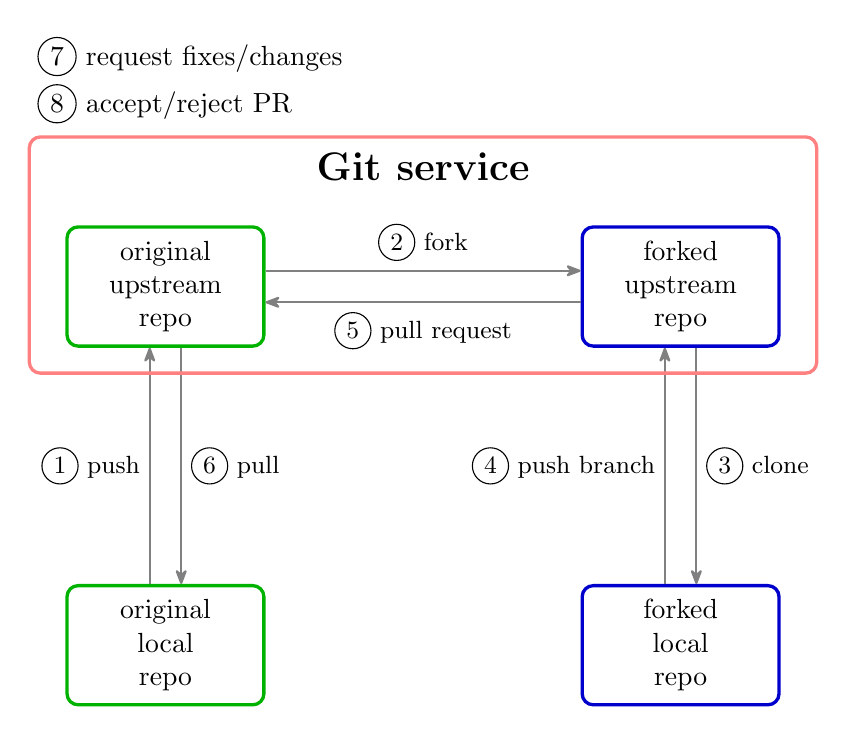
\begin{tikzpicture}
    \matrix [row sep=30mm, column sep=40mm] {%
        \node[repo, draw=green!70!black] (ownerupstream) {original\\upstream\\repo}; &
        \node[repo, draw=blue!80!black] (forkedupstream) {forked\\upstream\\repo};\\

        \node[repo, draw=green!70!black] (ownerlocal) {original\\local\\repo}; &
        \node[repo, draw=blue!80!black] (forkedlocal) {forked\\local\\repo};\\
    };

    \coordinate (olpush) at ($(ownerlocal.north) - (0.2,0)$);
    \coordinate (oupush) at ($(ownerupstream.south) - (0.2,0)$);

    \coordinate (olpull) at ($(ownerlocal.north) + (0.2,0)$);
    \coordinate (oupull) at ($(ownerupstream.south) + (0.2,0)$);

    \coordinate (oufork) at ($(ownerupstream.east) + (0, 0.2)$);
    \coordinate (fufork) at ($(forkedupstream.west) + (0, 0.2)$);

    \coordinate (oupr) at ($(ownerupstream.east) - (0, 0.2)$);
    \coordinate (fupr) at ($(forkedupstream.west) - (0, 0.2)$);

    \coordinate (fuclone) at ($(forkedupstream.south) + (0.2, 0)$);
    \coordinate (flclone) at ($(forkedlocal.north) + (0.2, 0)$);

    \coordinate (fupush) at ($(forkedupstream.south) - (0.2, 0)$);
    \coordinate (flpush) at ($(forkedlocal.north) - (0.2, 0)$);

    \draw[prarrow, ->] (olpush) -- (oupush) node[prstep, left] {\circled{1} push};
    \draw[prarrow, ->] (oupull) -- (olpull) node[prstep, right] {\circled{6} pull};

    \draw[prarrow, ->] (oufork) -- (fufork) node[prstep, above] {\circled{2} fork};
    \draw[prarrow, ->] (fupr) -- (oupr) node[prstep, below] {\circled{5} pull request};

    \draw[prarrow, ->] (fuclone) -- (flclone) node[prstep, right] {\circled{3} clone};
    \draw[prarrow, ->] (flpush) -- (fupush) node[prstep, left] {\circled{4} push branch};

    \node[
        draw=red!50,
        very thick,
        rounded corners,
        minimum width=100mm,
        minimum height=30mm,
    ] (gitservice) at ($(oufork)!0.5!(fufork) + (0, 0.2)$) {};
    \node at ($(gitservice.north) + (0, -0.4)$) {\Large \textbf{Git service}};
    \node[anchor=west] at ($(gitservice.north west) + (0, 1.0)$) {\circled{7} request fixes/changes};
    \node[anchor=west] at ($(gitservice.north west) + (0, 0.4)$) {\circled{8} accept/reject PR};
\end{tikzpicture}

\end{document}
